% Created 2023-01-02 Mon 21:15
\documentclass[9pt, b5paper]{article}
\usepackage{xeCJK}
\usepackage{minted}
\usepackage[T1]{fontenc}
\usepackage[scaled]{beraserif}
\usepackage[scaled]{berasans}
\usepackage[scaled]{beramono}
\usepackage{graphicx}
\usepackage{xcolor}
\usepackage{multirow}
\usepackage{multicol}
\usepackage{float}
\usepackage{textcomp}
\usepackage{algorithm}
\usepackage{algorithmic}
\usepackage{latexsym}
\usepackage{natbib}
\usepackage{geometry}
\geometry{left=1.2cm,right=1.2cm,top=1.5cm,bottom=1.2cm}
\newminted{common-lisp}{fontsize=\footnotesize} 
\usepackage[xetex,colorlinks=true,CJKbookmarks=true,linkcolor=blue,urlcolor=blue,menucolor=blue]{hyperref}
\author{deepwaterooo}
\date{\today}
\title{手机游戏平台热更新服务器--一个实例学习笔记GeekServer}
\hypersetup{
  pdfkeywords={},
  pdfsubject={},
  pdfcreator={Emacs 27.2 (Org mode 8.2.7c)}}
\begin{document}

\maketitle
\tableofcontents


\section{手机游戏平台热更新服务器--一个实例学习笔记}
\label{sec-1}
\begin{itemize}
\item 到现在为止,基本上只找到了这一个自己可以运行的本地热更新服务器的框架.所源码基本上都读了一遍,但因为对自己来说服务器是完全陌生的领域,它读起来甚至比ET框架难多了,有不少不熟悉的概念与原理,比如Actor, TCP WebSocket等。这个框架可能学习curve会稍微陡峭一点儿,涉及到的尖端知识点比较多,比如用的是RocksDB等,很多原理自己会一一学习掌握
\item 但因为它能够运行,今天下午终于能够看进改掉visual studio 2019终端显示中文的问题.就再从运行日志入手,借助日志,把这个本地服务器弄得再明白一点儿后,准备开始着手写自己最简单的热更新服务器.
\item 这里的本地热更新服务器,与项目中游戏里的游戏客户端,接下来会需要从两端都运行,来分析学习源码.先从服务器入手
\item 现在才明白,这个框架更多的是支持服务器的热更新,与自已想要实现的最简单的相差狠远。我基本可以不需要热更新我的安卓平台客户端游戏的热更新服务器。
\end{itemize}

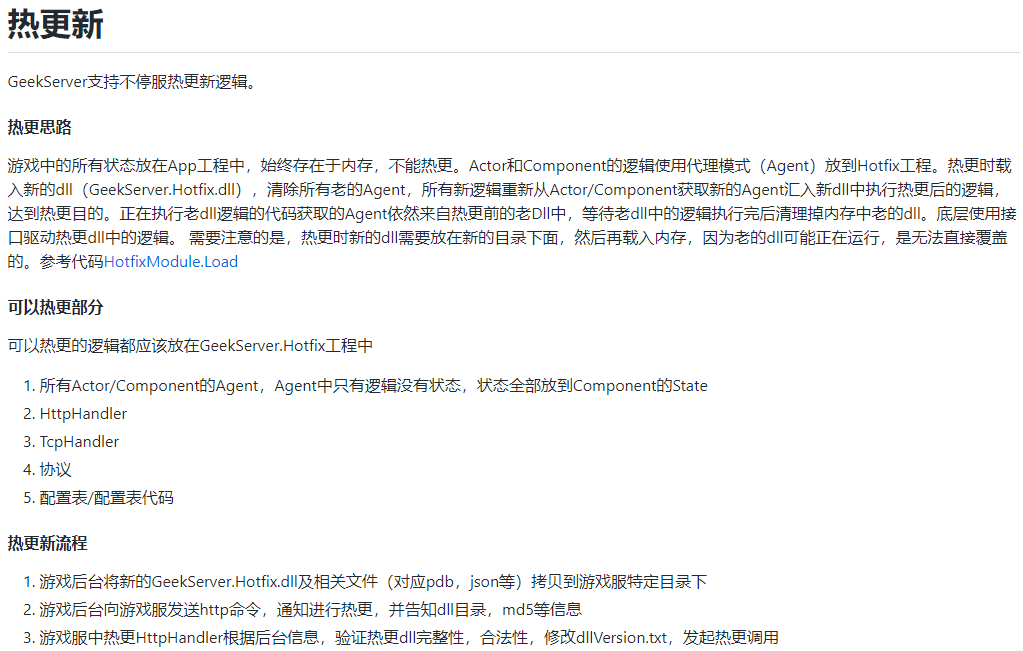
\includegraphics[width=.9\linewidth]{./pic/readme_20230102_205637.png}
\begin{itemize}
\item 因为同自已的项目需要,还是相差得比较远,所以这个项目暂时也还是放一下。但任何时候都可以成为学习的资源再深化理解一下。 
\begin{itemize}
\item 热更思路: 这是关于服务器热更新的逻辑,我基本上用不到,我现在可以不用考虑服务器的热更新,只要客户端的游戏可以热更新就可以了
\begin{itemize}
\item 游戏中的所有状态放在App工程中,始终存在于内存,不能热更。Actor和Component的逻辑使用代理模式(Agent)放到Hotfix工程。热更时载入新的dll(GeekServer.Hotfix.dll),清除所有老的Agent,所有新逻辑重新从Actor/Component获取新的Agent汇入新dll中执行热更后的逻辑,达到热更目的。正在执行老dll逻辑的代码获取的Agent依然来自热更前的老Dll中,等待老dll中的逻辑执行完后清理掉内存中老的dll。底层使用接口驱动热更dll中的逻辑。 需要注意的是,热更时新的dll需要放在新的目录下面,然后再载入内存,因为老的dll可能正在运行,是无法直接覆盖的。参考代码HotfixModule.Load
\end{itemize}
\item 可以热更部分
\begin{itemize}
\item 位置:可以热更的逻辑都应该放在GeekServer.Hotfix工程中
\item 所有Actor/Component的Agent,Agent中只有逻辑没有状态,状态全部放到Component的State
\item HttpHandler
\item TcpHandler
\item 协议
\item 配置表/配置表代码
\end{itemize}

\item 热更新流程
\begin{itemize}
\item 游戏后台将新的GeekServer.Hotfix.dll及相关文件(对应pdb,json等)拷贝到游戏服特定目录下
\item 游戏后台向游戏服发送http命令,通知进行热更,并告知dll目录,md5等信息
\item 游戏服中热更HttpHandler根据后台信息,验证热更dll完整性,合法性,修改dllVersion.txt,发起热更调用
\end{itemize}
\end{itemize}
\end{itemize}
\#+END\_SRC
\begin{itemize}
\item 所以是,一不小心,读了一个好难的服务器热更新的框架源码!虽然明确感受到learning curve一下子猛增,但还是收获狠多的。以后爬爬源码什么的会感觉轻松无压力。。。。。爱表哥,爱生活!!!
\end{itemize}

\begin{minted}[fontsize=\scriptsize,linenos=false]{text}
init NLog config...
***PolymorphicRegister Init***
 INFO  launch embedded db...
 INFO  regist comps...
 INFO  初始化组件注册完成
 INFO  load hotfix module
LoadHotfixModule: reload = False
 INFO  hotfix dll init success: F:\unityGamesExamples\GeekServer\bin\app_debug\hotfix/Geek.Server.Hotfix.dll
HotfixMgr (module.HotfixBridge != null) = True

// <<<<<<<<<< 我找不到下面这些是从哪里来,不知道是不是什么第三方库的.dll程序集里出来的,又或者是数据库 ? .NET Core WEB ?

// 感觉这是 TcpServer WebApplication创建时,内部生成的, 其内部创建实现原理不是很懂
 DEBUG  Hosting starting
 INFO  Now listening on: http://[::]:8899
 DEBUG  Loaded hosting startup assembly Geek.Server.App
 INFO  Application started. Press Ctrl+C to shut down.
 INFO  Hosting environment: Production
 INFO  Content root path: F:\unityGamesExamples\GeekServer\bin\app_debug\
 DEBUG  Hosting started
 INFO  tcp 服务启动完成... 这里,这一行可以找到
HotfixBridge tcp 服务启动完成...

// 感觉这是 HttpServer WebApplication创建时,内部生成的, 其内部创建实现原理不是很懂
 DEBUG  Hosting starting
 INFO  Now listening on: http://[::]:20000
 DEBUG  Loaded hosting startup assembly Geek.Server.App
 INFO  Application started. Press Ctrl+C to shut down.
 INFO  Hosting environment: Production
 INFO  Content root path: F:\unityGamesExamples\GeekServer\bin\app_debug\
 DEBUG  Hosting started

 INFO  load config data
 INFO  初始化全局定时完成
 INFO  下次定时回存时间 1/2/2023 11:10:09 AM
 INFO  激活全局Actor: Server
 INFO  激活全局组件并检测组件是否都包含Agent实现完成

 INFO  进入游戏主循环...
        ***进入游戏主循环***

// 下面这两行日志好像又找不到了
 DEBUG  ServerCompAgent.TestSchedueTimer.延时1秒执行.每隔30秒执行
 DEBUG  ServerCompAgent.TestDelayTimer.延时3秒执行.执行一次
 DEBUG  Connection id "0HMNCUJ22HQ5P" accepted.
 DEBUG  Connection id "0HMNCUJ22HQ5P" started.
 DEBUG  [::ffff:127.0.0.1]:62275 链接成功
 DEBUG  PetCompAgent.OnGotNewPet监听到了获得宠物的事件,宠物ID:1000当前世界等级:1

 DEBUG  ServerCompAgent.TestSchedueTimer.延时1秒执行.每隔30秒执行
 DEBUG  ServerCompAgent.TestSchedueTimer.延时1秒执行.每隔30秒执行
 DEBUG  ServerCompAgent.TestSchedueTimer.延时1秒执行.每隔30秒执行
 INFO  定时回存完成 耗时: 6.4955ms
 INFO  下次定时回存时间 1/2/2023 11:15:09 AM
 DEBUG  ServerCompAgent.TestSchedueTimer.延时1秒执行.每隔30秒执行
 DEBUG  ServerCompAgent.TestSchedueTimer.延时1秒执行.每隔30秒执行
 DEBUG  ServerCompAgent.TestSchedueTimer.延时1秒执行.每隔30秒执行
 DEBUG  ServerCompAgent.TestSchedueTimer.延时1秒执行.每隔30秒执行
 DEBUG  ServerCompAgent.TestSchedueTimer.延时1秒执行.每隔30秒执行
 DEBUG  ServerCompAgent.TestSchedueTimer.延时1秒执行.每隔30秒执行
 DEBUG  ServerCompAgent.TestSchedueTimer.延时1秒执行.每隔30秒执行
 DEBUG  ServerCompAgent.TestSchedueTimer.延时1秒执行.每隔30秒执行
 DEBUG  ServerCompAgent.TestSchedueTimer.延时1秒执行.每隔30秒执行
 DEBUG  ServerCompAgent.TestSchedueTimer.延时1秒执行.每隔30秒执行
 INFO  定时回存完成 耗时: 0.0761ms
 INFO  下次定时回存时间 1/2/2023 11:20:09 AM

// 当客户端断开连接之后
 DEBUG  Connection id "0HMNCUJ22HQ5P" received FIN.
 DEBUG  [::ffff:127.0.0.1]:62275 断开链接
 DEBUG  Connection id "0HMNCUJ22HQ5P" stopped.
 DEBUG  Connection id "0HMNCUJ22HQ5P" sending FIN because: "The Socket transport's send loop completed gracefully."
 DEBUG  ServerCompAgent.TestSchedueTimer.延时1秒执行.每隔30秒执行

// 当服务端关掉之后
F:\unityGamesExamples\GeekServer\bin\app_debug\Geek.Server.App.exe (process 13744) exited with code -1.
To automatically close the console when debugging stops, enable Tools->Options->Debugging->Automatically close the console when debugging stops.
Press any key to close this window . . . 
\end{minted}
\begin{itemize}
\item unity游戏客户端的部分
\end{itemize}

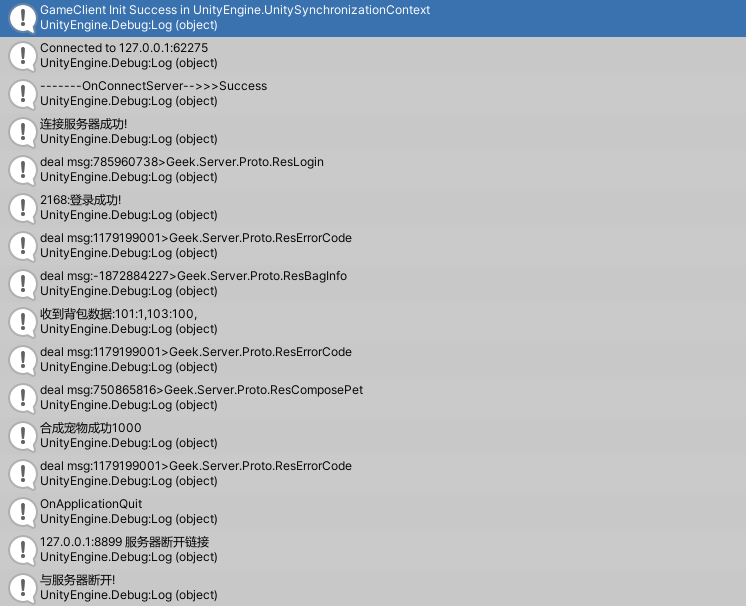
\includegraphics[width=.9\linewidth]{./pic/readme_20230102_111227.png}

\begin{minted}[fontsize=\scriptsize,linenos=false]{tex}
GameClient Init Success in UnityEngine.UnitySynchronizationContext
UnityEngine.Debug:Log (object)
Geek.Client.GameClient:Init () (at Assets/Scripts/Framework/Net/GameClient.cs:33)
Logic.GameMain/<Start>d__7:MoveNext () (at Assets/Scripts/Logic/GameMain.cs:28)

Connected to 127.0.0.1:62275 // 这里感觉是服务器里的日志,找不到
UnityEngine.Debug:Log (object)
Geek.Client.GameClient/<Connect>d__23:MoveNext () (at Assets/Scripts/Framework/Net/GameClient.cs:60)
UnityEngine.UnitySynchronizationContext:ExecuteTasks ()

-------OnConnectServer-->>>Success
UnityEngine.Debug:Log (object)
Logic.DemoService:OnConnectServer (Geek.Client.Event) (at Assets/Scripts/Logic/DemoService.cs:83)

连接服务器成功!
UnityEngine.Debug:Log (object)
Logic.DemoService:OnConnectServer (Geek.Client.Event) (at Assets/Scripts/Logic/DemoService.cs:86)

deal msg:785960738>Geek.Server.Proto.ResLogin // <<<<<<<<<<<<<<<<<<<< 这里是从哪里来的  
UnityEngine.Debug:Log (object)
Logic.DemoService:GetCurMsg<Geek.Server.Proto.ResLogin> (int) (at Assets/Scripts/Logic/DemoService.cs:51)

2678:登录成功! // 这个号不知道哪里来的
UnityEngine.Debug:Log (object)
Logic.DemoService:OnResLogin (Geek.Client.Event) (at Assets/Scripts/Logic/DemoService.cs:99)

deal msg:1179199001>Geek.Server.Proto.ResErrorCode
UnityEngine.Debug:Log (object)
Logic.DemoService:GetCurMsg<Geek.Server.Proto.ResErrorCode> (int) (at Assets/Scripts/Logic/DemoService.cs:51)

deal msg:-1872884227>Geek.Server.Proto.ResBagInfo
UnityEngine.Debug:Log (object)
Logic.DemoService:GetCurMsg<Geek.Server.Proto.ResBagInfo> (int) (at Assets/Scripts/Logic/DemoService.cs:51)

收到背包数据:101:1,103:100,
UnityEngine.Debug:Log (object)
Logic.DemoService:OnResBagInfo (Geek.Client.Event) (at Assets/Scripts/Logic/DemoService.cs:110)

deal msg:1179199001>Geek.Server.Proto.ResErrorCode
UnityEngine.Debug:Log (object)
Logic.DemoService:GetCurMsg<Geek.Server.Proto.ResErrorCode> (int) (at Assets/Scripts/Logic/DemoService.cs:51)

deal msg:750865816>Geek.Server.Proto.ResComposePet
UnityEngine.Debug:Log (object)
Logic.DemoService:GetCurMsg<Geek.Server.Proto.ResComposePet> (int) (at Assets/Scripts/Logic/DemoService.cs:51)

合成宠物成功1000
UnityEngine.Debug:Log (object)
Logic.DemoService:OnResComposePet (Geek.Client.Event) (at Assets/Scripts/Logic/DemoService.cs:116)

deal msg:1179199001>Geek.Server.Proto.ResErrorCode
UnityEngine.Debug:Log (object)
Logic.DemoService:GetCurMsg<Geek.Server.Proto.ResErrorCode> (int) (at Assets/Scripts/Logic/DemoService.cs:51)

OnApplicationQuit
UnityEngine.Debug:Log (object)
Logic.GameMain:OnApplicationQuit () (at Assets/Scripts/Logic/GameMain.cs:70)

127.0.0.1:8899 服务器断开链接
UnityEngine.Debug:Log (object)
Geek.Client.NetChannel:ConnectionClosed () (at Assets/Scripts/Framework/Net/NetChannel.cs:26)
Geek.Client.ClientNetChannel:ConnectionClosed () (at Assets/Scripts/Framework/Net/ClientNetChannel.cs:19)

与服务器断开!
UnityEngine.Debug:Log (object)
Logic.DemoService:OnDisconnectServer (Geek.Client.Event) (at Assets/Scripts/Logic/DemoService.cs:94)
\end{minted}

\begin{itemize}
\item HotfixBridge.cs: 服务器端:这里分两块初始化的代码主要来自于服务器热更新中的代码:
\end{itemize}
\begin{minted}[fontsize=\scriptsize,linenos=false]{csharp}
namespace Server.Logic.Common {

    internal class HotfixBridge : IHotfixBridge {
        private const string TAG = "HotfixBridge";

        private static readonly Logger Log = LogManager.GetCurrentClassLogger();
        public ServerType BridgeType => ServerType.Game;

        public async Task<bool> OnLoadSuccess(bool reload) { // 当程序集启动完成之后 的回调
            Console.WriteLine(TAG + "OnLoadSuccess() reload = " + reload);
            if (reload) {
                ActorMgr.ClearAgent();
                return true;
            }
            PolymorphicTypeMapper.Register(this.GetType().Assembly);
            HotfixMgr.SetMsgGetter(MsgFactory.GetType);

// <<<<<<<<<<<<<<<<<<<< 
            // await TcpServer.Start(Settings.TcpPort);
            await TcpServer.Start(Settings.TcpPort, builder => builder.UseConnectionHandler<AppTcpConnectionHandler>());
            Log.Info("tcp 服务启动完成...");

// <<<<<<<<<<<<<<<<<<<< 
            await HttpServer.Start(Settings.HttpPort);

// <<<<<<<<<<<<<<<<<<<< 
            Log.Info("load config data");
            (bool success, string msg) = GameDataManager.ReloadAll();
            if (!success)
                throw new Exception($"载入配置表失败... {msg}");
            GlobalTimer.Start();
            await CompRegister.ActiveGlobalComps();
            return true;
        }

        public async Task Stop() {
            // 断开所有连接
            await SessionManager.RemoveAll();
            // 取消所有未执行定时器
            await QuartzTimer.Stop();
            // 保证actor之前的任务都执行完毕
            await ActorMgr.AllFinish();
            // 关闭网络服务
            await HttpServer.Stop();
            await TcpServer.Stop();
            // 存储所有数据
            await GlobalTimer.Stop();
            await ActorMgr.RemoveAll();
        }
    }
}
\end{minted}
\begin{itemize}
\item 客户端:
\end{itemize}

\section{TcpServer}
\label{sec-2}
\begin{itemize}
\item 有些是系统里的类和方法:比如下面的:
\end{itemize}
\section{IHost.cs}
\label{sec-3}

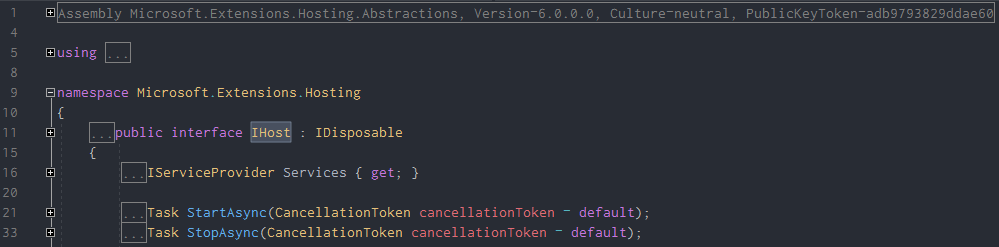
\includegraphics[width=.9\linewidth]{./pic/readme_20230101_222709.png}
\begin{itemize}
\item 这里,WebApplication的内部创建实现原理不是很懂
\end{itemize}

\section{AppStartUp: 负责服务器的启动}
\label{sec-4}
\begin{minted}[fontsize=\scriptsize,linenos=false]{csharp}
internal class AppStartUp {

    static readonly Logger Log = LogManager.GetCurrentClassLogger();

    public static async Task Enter() {
        try {
            var flag = Start(); // <<<<<<<<<<<<<<<<<<<< 
            if (!flag) return; // 启动服务器失败
            Log.Info($"launch embedded db...");
            ActorLimit.Init(ActorLimit.RuleType.None);
            GameDB.Init();
            GameDB.Open();
            Log.Info($"regist comps...");
            await CompRegister.Init();

            Log.Info($"load hotfix module");
            await HotfixMgr.LoadHotfixModule();

            Log.Info("进入游戏主循环...");
            Console.WriteLine("***进入游戏主循环***");

            Settings.LauchTime = DateTime.Now;
            Settings.AppRunning = true;
            TimeSpan delay = TimeSpan.FromSeconds(1);
            while (Settings.AppRunning) {
                await Task.Delay(delay);
            }
        }
        catch (Exception e) {
            Console.WriteLine($"服务器执行异常,e:{e}");
            Log.Fatal(e);
        }
        Console.WriteLine($"退出服务器开始");
        await HotfixMgr.Stop();
        Console.WriteLine($"退出服务器成功");
    }

    private static bool Start() { // <<<<<<<<<<<<<<<<<<<< 
        try {
            Settings.Load<AppSetting>("Configs/app_config.json", ServerType.Game); // 服务器的配置文件 

            Console.WriteLine("init NLog config..."); // 配置日志系统: CPU/IO 密集型的服务器,日志就显示狠复杂[暂放一下]
            LayoutRenderer.Register<NLogConfigurationLayoutRender>("logConfiguration");
            LogManager.Configuration = new XmlLoggingConfiguration("Configs/app_log.config");
            LogManager.AutoShutdown = false;

            PolymorphicTypeMapper.Register(typeof(AppStartUp).Assembly); // app
            PolymorphicRegister.Load();
            PolymorphicResolver.Init();
            return true;
        }
        catch (Exception e) {
            Log.Error($"启动服务器失败,异常:{e}");
            return false;
        }
    }
}
\end{minted}
\section{服务器的配置文件 Configs/app\_config.json}
\label{sec-5}

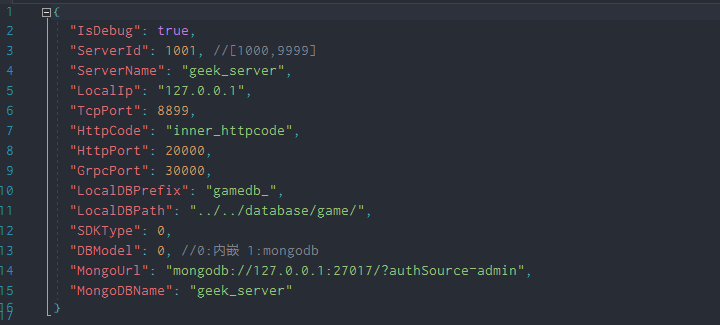
\includegraphics[width=.9\linewidth]{./pic/readme_20230101_180011.png}
\begin{minted}[fontsize=\scriptsize,linenos=false]{tex}
{
  "IsDebug": true,
  "ServerId": 1001, //[1000,9999]
  "ServerName": "geek_server",
  "LocalIp": "127.0.0.1",
  "TcpPort": 8899,
  "HttpCode": "inner_httpcode",
  "HttpPort": 20000,
  "GrpcPort": 30000,
  "LocalDBPrefix": "gamedb_",
  "LocalDBPath": "../../database/game/",
  "SDKType": 0,
  "DBModel": 0, //0:内嵌 1:mongodb
  "MongoUrl": "mongodb://127.0.0.1:27017/?authSource=admin",
  "MongoDBName": "geek_server"
}
\end{minted}

\section{TaskCompletionSource.cs}
\label{sec-6}
\begin{minted}[fontsize=\scriptsize,linenos=false]{csharp}
namespace System.Threading.Tasks
{
    public class TaskCompletionSource<TResult>
    {
        public TaskCompletionSource();
        public TaskCompletionSource(object state);
        public TaskCompletionSource(TaskCreationOptions creationOptions);
        public TaskCompletionSource(object state, TaskCreationOptions creationOptions);

        public Task<TResult> Task { get; }

        public void SetCanceled();
        public void SetException(IEnumerable<Exception> exceptions);
        public void SetException(Exception exception);
        public void SetResult(TResult result);
        public bool TrySetCanceled();
        public bool TrySetCanceled(CancellationToken cancellationToken);
        public bool TrySetException(IEnumerable<Exception> exceptions);
        public bool TrySetException(Exception exception);
        public bool TrySetResult(TResult result);
    }
}
\end{minted}
\section{GameClient.cs}
\label{sec-7}
\begin{itemize}
\item async Task<ClientNetChannel> Connect(string host, int port) : 与远程服务器连接的部分
\end{itemize}
\begin{minted}[fontsize=\scriptsize,linenos=false]{csharp}
public int Port { private set; get; }
public string Host { private set; get; }
public const int ConnectEvt = 101; // 连接事件
public const int DisconnectEvt = 102; // 连接断开

public async Task<ClientNetChannel> Connect(string host, int port) {
    Host = host;
    Port = port;
    try {
        var connection = await ClientFactory.ConnectAsync(new IPEndPoint(IPAddress.Parse(Host), Port)); // 异步连接
        UnityEngine.Debug.Log($"Connected to {connection.LocalEndPoint}");
        Channel = new ClientNetChannel(connection, new ClientLengthPrefixedProtocol());
        OnConnected(NetCode.Success);
        return Channel;
    }
    catch (Exception e) {
        UnityEngine.Debug.LogError(e.ToString());
        OnConnected(NetCode.Failed);
        throw;
    }
}
\end{minted}
\begin{itemize}
\item ClientFactory.cs再往底层一点儿的细节
\begin{minted}[fontsize=\scriptsize,linenos=false]{csharp}
public static class ClientFactory {

    public static async ValueTask<ConnectionContext> ConnectAsync(EndPoint endpoint) {
        var conn = new SocketConnection(endpoint).StartAsync(); // <<<<<<<<<< 
        return await conn.ConfigureAwait(false);
    }
}
\end{minted}
\item SocketConnection.cs : ConnectionContext
\end{itemize}
\begin{minted}[fontsize=\scriptsize,linenos=false]{csharp}
public async ValueTask<ConnectionContext> StartAsync() {
    await _socket.ConnectAsync(_endPoint).ConfigureAwait(false); // <<<<<<<<<<  
    var pair = DuplexPipe.CreateConnectionPair(PipeOptions.Default, PipeOptions.Default);
    LocalEndPoint = _socket.LocalEndPoint;
    RemoteEndPoint = _socket.RemoteEndPoint;
    Transport = pair.Transport;
    _application = pair.Application;
    _ = ExecuteAsync(); // <<<<<<<<<< 
    return this;
}
private async Task ExecuteAsync() {
    Exception sendError = null;
    try {
        // Spawn send and receive logic
        var receiveTask = DoReceive();
        var sendTask = DoSend();
        // If the sending task completes then close the receive
        // We don't need to do this in the other direction because the kestrel
        // will trigger the output closing once the input is complete.
        if (await Task.WhenAny(receiveTask, sendTask).ConfigureAwait(false) == sendTask) { // 这里什么情况下等,读得稀里糊涂
            // Tell the reader it's being aborted
            _socket.Dispose();
        }
        // Now wait for both to complete
        await receiveTask;
        sendError = await sendTask;
        // Dispose the socket(should noop if already called)
        _socket.Dispose();
    }
    catch (Exception ex) {
        Console.WriteLine($"Unexpected exception in {nameof(SocketConnection)}.{nameof(StartAsync)}: " + ex);
    }
    finally {
        // Complete the output after disposing the socket
        _application.Input.Complete(sendError);
    }
}
\end{minted}
\begin{itemize}
\item 
\end{itemize}
% Emacs 27.2 (Org mode 8.2.7c)
\end{document}